\documentclass[tikz,border=7pt]{standalone}
\usepackage{iftex}
\ifPDFTeX
  \PackageError{matrix-figure}{This figure requires XeTeX or Tectonic}{Compile with xelatex or tectonic.}
\fi
\usepackage{fontspec}
\usepackage{xeCJK}
\usepackage{amsmath}
\usepackage{unicode-math}
\usepackage{xcolor}
\usepackage{tikz}
\usetikzlibrary{arrows.meta,positioning}

\providecommand{\FigureUseLocalFonts}{0}
\ifnum\FigureUseLocalFonts=1
  \setmainfont{NotoSansCJKtc-Regular.otf}[Path=\FigureSansFontPath]
  \setsansfont{NotoSansCJKtc-Regular.otf}[Path=\FigureSansFontPath,BoldFont=NotoSansCJKtc-Bold.otf]
  \setCJKmainfont{NotoSansCJKtc-Regular.otf}[Path=\FigureSansFontPath]
  \setCJKsansfont{NotoSansCJKtc-Regular.otf}[Path=\FigureSansFontPath,BoldFont=NotoSansCJKtc-Bold.otf]
  \setmathfont{STIXTwoMath.otf}[Path=\FigureMathFontPath]
\else
  \setmainfont{Noto Sans CJK TC}
  \setsansfont{Noto Sans CJK TC}
  \setCJKmainfont{Noto Sans CJK TC}
  \setCJKsansfont{Noto Sans CJK TC}
  \setmathfont{STIX Two Math}
\fi

\definecolor{FigureInk}{HTML}{253142}
\definecolor{PanelFill}{gray}{0.96}
\definecolor{RowShade}{gray}{0.86}
\definecolor{ColumnShade}{gray}{0.74}
\definecolor{ResultShade}{gray}{0.58}
\definecolor{FocusShade}{gray}{0.68}
\definecolor{GuideShade}{gray}{0.80}

\newcommand{\MatrixCell}[2]{%
  \tikz[baseline=(value.base)]{\node[fill=#1,rounded corners=0.4pt,inner sep=2.2pt,
    minimum width=1.35em,minimum height=1.35em] (value) {$#2$};}%
}
\newcommand{\RowCell}[1]{\MatrixCell{RowShade}{#1}}
\newcommand{\ColumnCell}[1]{\MatrixCell{ColumnShade}{#1}}
\newcommand{\ResultCell}[1]{\MatrixCell{ResultShade}{#1}}
\newcommand{\FocusCell}[1]{\MatrixCell{FocusShade}{#1}}

\tikzset{
  figure/.style={font=\sffamily,text=FigureInk,>={Stealth[length=3.5mm,width=2.5mm]}},
  panel/.style={draw=FigureInk,line width=0.9pt,rounded corners=1.5mm,fill=PanelFill,align=center},
  flow/.style={-{Stealth},line width=1.05pt,draw=FigureInk},
}


\begin{document}
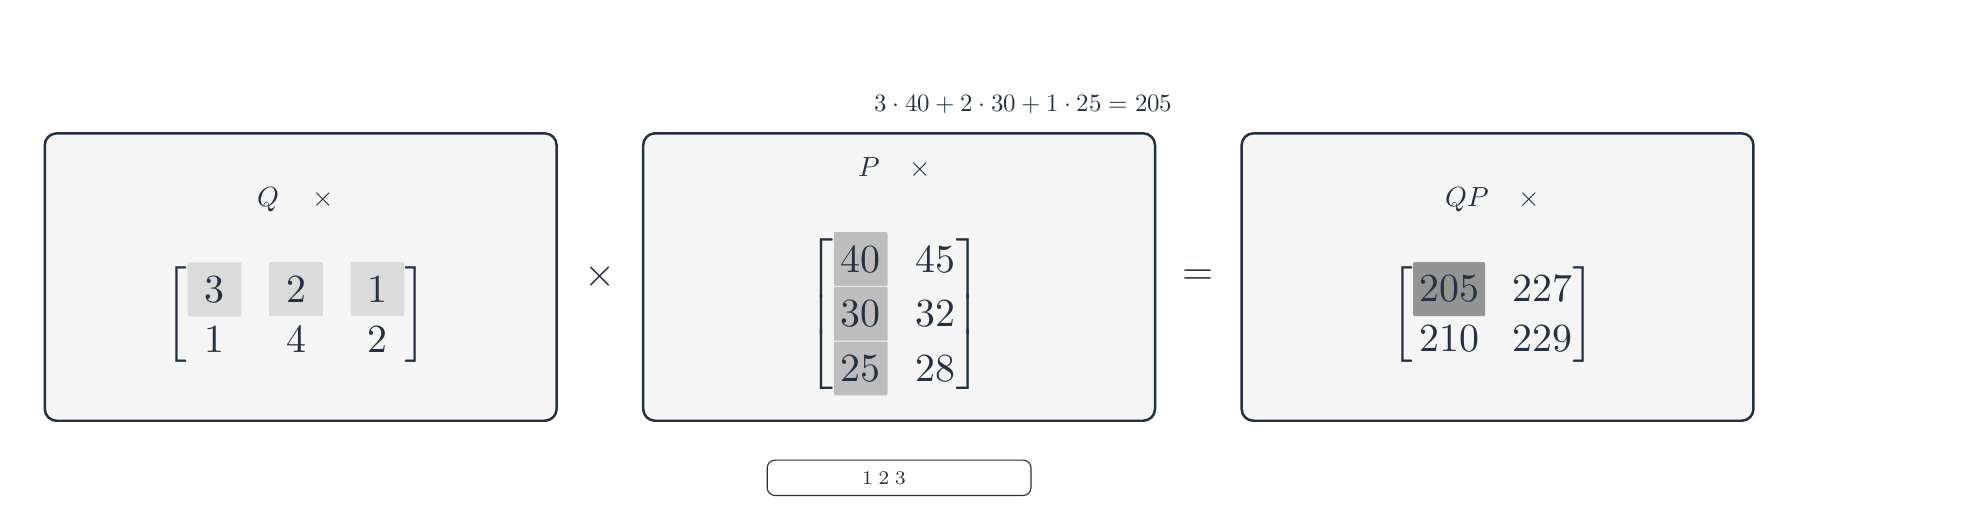
\begin{tikzpicture}[figure]
  \node[font=\bfseries\Large,align=center,text width=24cm] at (12,6.05)
    {共同的品項索引在乘法中被加總，結果保留學生與商店索引};
  \node[font=\small] at (12,5.2)
    {第一位學生在甲店的總價：$3\cdot40+2\cdot30+1\cdot25=205$};

  \node[panel,minimum width=6.5cm,minimum height=3.65cm] (Q) at (3.35,3.0) {%
    \begin{minipage}{5.9cm}\centering
      \textbf{數量 $Q$：學生 $\times$ 品項}\\[5pt]
      \scriptsize 行依序為三種品項\\[6pt]
      \Large$\begin{bmatrix}
        \RowCell{3}&\RowCell{2}&\RowCell{1}\\
        1&4&2
      \end{bmatrix}$
    \end{minipage}
  };
  \node[font=\Large] at (7.15,3.0) {$\times$};
  \node[panel,minimum width=6.5cm,minimum height=3.65cm] (P) at (10.95,3.0) {%
    \begin{minipage}{5.9cm}\centering
      \textbf{單價 $P$：品項 $\times$ 商店}\\[5pt]
      \scriptsize 列依序為三種品項\\[6pt]
      \Large$\begin{bmatrix}
        \ColumnCell{40}&45\\
        \ColumnCell{30}&32\\
        \ColumnCell{25}&28
      \end{bmatrix}$
    \end{minipage}
  };
  \node[font=\Large] at (14.75,3.0) {$=$};
  \node[panel,minimum width=6.5cm,minimum height=3.65cm] (QP) at (18.55,3.0) {%
    \begin{minipage}{5.9cm}\centering
      \textbf{總價 $QP$：學生 $\times$ 商店}\\[5pt]
      \scriptsize 每格是一位學生在一家商店的總價\\[6pt]
      \Large$\begin{bmatrix}
        \ResultCell{205}&227\\
        210&229
      \end{bmatrix}$
    \end{minipage}
  };

  \node[draw=FigureInk,rounded corners=1mm,fill=white,inner xsep=8pt,inner ysep=4pt,
        font=\scriptsize] at (10.95,0.45)
    {三個配對位置依序都是餐點 1、2、3；相乘後只留下學生與商店兩個外側索引。};
\end{tikzpicture}
\end{document}
